\chapter{The Night}

Monte Cristo waited, according to his usual custom, until Duprez had
sung his famous “\textit{Suivez-moi!}” then he rose and went out. Morrel took
leave of him at the door, renewing his promise to be with him the next
morning at seven o’clock, and to bring Emmanuel. Then he stepped into
his \textit{coupé}, calm and smiling, and was at home in five minutes. No one
who knew the count could mistake his expression when, on entering, he
said:

“Ali, bring me my pistols with the ivory cross.”

Ali brought the box to his master, who examined the weapons with a
solicitude very natural to a man who is about to intrust his life to a
little powder and shot. These were pistols of an especial pattern,
which Monte Cristo had had made for target practice in his own room. A
cap was sufficient to drive out the bullet, and from the adjoining room
no one would have suspected that the count was, as sportsmen would say,
keeping his hand in.

He was just taking one up and looking for the point to aim at on a
little iron plate which served him as a target, when his study door
opened, and Baptistin entered. Before he had spoken a word, the count
saw in the next room a veiled woman, who had followed closely after
Baptistin, and now, seeing the count with a pistol in his hand and
swords on the table, rushed in. Baptistin looked at his master, who
made a sign to him, and he went out, closing the door after him.

“Who are you, madame?” said the count to the veiled woman.

\begin{figure}[ht]
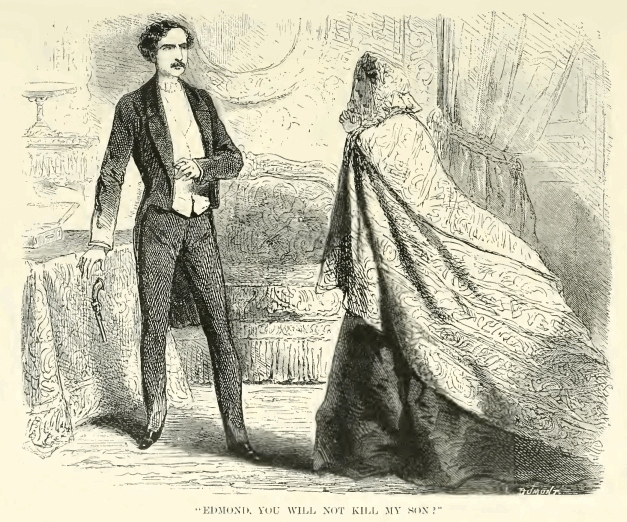
\includegraphics[width=\textwidth]{40227m.jpg}
\end{figure}

The stranger cast one look around her, to be certain that they were
quite alone; then bending as if she would have knelt, and joining her
hands, she said with an accent of despair:

“Edmond, you will not kill my son!”

The count retreated a step, uttered a slight exclamation, and let fall
the pistol he held.

“What name did you pronounce then, Madame de Morcerf?” said he.

“Yours!” cried she, throwing back her veil,—“yours, which I alone,
perhaps, have not forgotten. Edmond, it is not Madame de Morcerf who is
come to you, it is Mercédès.”

“Mercédès is dead, madame,” said Monte Cristo; “I know no one now of
that name.”

“Mercédès lives, sir, and she remembers, for she alone recognized you
when she saw you, and even before she saw you, by your voice,
Edmond,—by the simple sound of your voice; and from that moment she has
followed your steps, watched you, feared you, and she needs not to
inquire what hand has dealt the blow which now strikes M. de Morcerf.”

“Fernand, do you mean?” replied Monte Cristo, with bitter irony; “since
we are recalling names, let us remember them all.” Monte Cristo had
pronounced the name of Fernand with such an expression of hatred that
Mercédès felt a thrill of horror run through every vein.

“You see, Edmond, I am not mistaken, and have cause to say, ‘Spare my
son!’”

“And who told you, madame, that I have any hostile intentions against
your son?”

“No one, in truth; but a mother has twofold sight. I guessed all; I
followed him this evening to the Opera, and, concealed in a parquet
box, have seen all.”

“If you have seen all, madame, you know that the son of Fernand has
publicly insulted me,” said Monte Cristo with awful calmness.

“Oh, for pity’s sake!”

“You have seen that he would have thrown his glove in my face if
Morrel, one of my friends, had not stopped him.”

“Listen to me, my son has also guessed who you are,—he attributes his
father’s misfortunes to you.”

“Madame, you are mistaken, they are not misfortunes,—it is a
punishment. It is not I who strike M. de Morcerf; it is Providence
which punishes him.”

“And why do you represent Providence?” cried Mercédès. “Why do you
remember when it forgets? What are Yanina and its vizier to you,
Edmond? What injury has Fernand Mondego done you in betraying Ali
Tepelini?”

“Ah, madame,” replied Monte Cristo, “all this is an affair between the
French captain and the daughter of Vasiliki. It does not concern me,
you are right; and if I have sworn to revenge myself, it is not on the
French captain, or the Count of Morcerf, but on the fisherman Fernand,
the husband of Mercédès the Catalane.”

“Ah, sir!” cried the countess, “how terrible a vengeance for a fault
which fatality made me commit!—for I am the only culprit, Edmond, and
if you owe revenge to anyone, it is to me, who had not fortitude to
bear your absence and my solitude.”

“But,” exclaimed Monte Cristo, “why was I absent? And why were you
alone?”

\begin{figure}[ht]
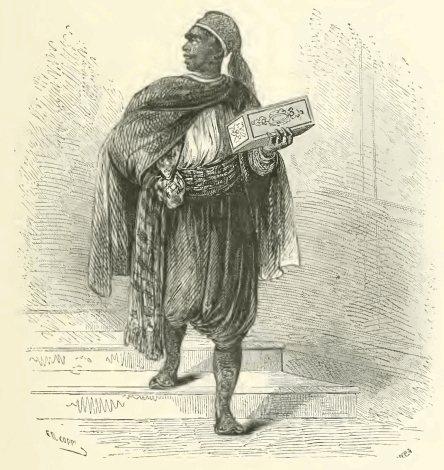
\includegraphics[width=\textwidth]{40231m.jpg}
\end{figure}

“Because you had been arrested, Edmond, and were a prisoner.”

“And why was I arrested? Why was I a prisoner?”

“I do not know,” said Mercédès.

“You do not, madame; at least, I hope not. But I will tell you. I was
arrested and became a prisoner because, under the arbor of La Réserve,
the day before I was to marry you, a man named Danglars wrote this
letter, which the fisherman Fernand himself posted.”

Monte Cristo went to a secretaire, opened a drawer by a spring, from
which he took a paper which had lost its original color, and the ink of
which had become of a rusty hue—this he placed in the hands of
Mercédès. It was Danglars’ letter to the king’s attorney, which the
Count of Monte Cristo, disguised as a clerk from the house of Thomson \&
French, had taken from the file against Edmond Dantès, on the day he
had paid the two hundred thousand francs to M. de Boville. Mercédès
read with terror the following lines:

\begin{quote}
{\small“The king’s attorney is informed by a friend to the throne and religion
that one Edmond Dantès, second in command on board the \textit{Pharaon}, this
day arrived from Smyrna, after having touched at Naples and
Porto-Ferrajo, is the bearer of a letter from Murat to the usurper, and
of another letter from the usurper to the Bonapartist club in Paris.
Ample corroboration of this statement may be obtained by arresting the
above-mentioned Edmond Dantès, who either carries the letter for Paris
about with him, or has it at his father’s abode. Should it not be found
in possession of either father or son, then it will assuredly be
discovered in the cabin belonging to the said Dantès on board the
\textit{Pharaon}.”}
\end{quote}

“How dreadful!” said Mercédès, passing her hand across her brow, moist
with perspiration; “and that letter——”

“I bought it for two hundred thousand francs, madame,” said Monte
Cristo; “but that is a trifle, since it enables me to justify myself to
you.”

“And the result of that letter——”

“You well know, madame, was my arrest; but you do not know how long
that arrest lasted. You do not know that I remained for fourteen years
within a quarter of a league of you, in a dungeon in the Château d’If.
You do not know that every day of those fourteen years I renewed the
vow of vengeance which I had made the first day; and yet I was not
aware that you had married Fernand, my calumniator, and that my father
had died of hunger!”

“Can it be?” cried Mercédès, shuddering.

“That is what I heard on leaving my prison fourteen years after I had
entered it; and that is why, on account of the living Mercédès and my
deceased father, I have sworn to revenge myself on Fernand, and—I have
revenged myself.”

“And you are sure the unhappy Fernand did that?”

“I am satisfied, madame, that he did what I have told you; besides,
that is not much more odious than that a Frenchman by adoption should
pass over to the English; that a Spaniard by birth should have fought
against the Spaniards; that a stipendiary of Ali should have betrayed
and murdered Ali. Compared with such things, what is the letter you
have just read?—a lover’s deception, which the woman who has married
that man ought certainly to forgive; but not so the lover who was to
have married her. Well, the French did not avenge themselves on the
traitor, the Spaniards did not shoot the traitor, Ali in his tomb left
the traitor unpunished; but I, betrayed, sacrificed, buried, have risen
from my tomb, by the grace of God, to punish that man. He sends me for
that purpose, and here I am.”

The poor woman’s head and arms fell; her legs bent under her, and she
fell on her knees.

“Forgive, Edmond, forgive for my sake, who love you still!”

The dignity of the wife checked the fervor of the lover and the mother.
Her forehead almost touched the carpet, when the count sprang forward
and raised her. Then seated on a chair, she looked at the manly
countenance of Monte Cristo, on which grief and hatred still impressed
a threatening expression.

“Not crush that accursed race?” murmured he; “abandon my purpose at the
moment of its accomplishment? Impossible, madame, impossible!”

“Edmond,” said the poor mother, who tried every means, “when I call you
Edmond, why do you not call me Mercédès?”

“Mercédès!” repeated Monte Cristo; “Mercédès! Well yes, you are right;
that name has still its charms, and this is the first time for a long
period that I have pronounced it so distinctly. Oh, Mercédès, I have
uttered your name with the sigh of melancholy, with the groan of
sorrow, with the last effort of despair; I have uttered it when frozen
with cold, crouched on the straw in my dungeon; I have uttered it,
consumed with heat, rolling on the stone floor of my prison. Mercédès,
I must revenge myself, for I suffered fourteen years,—fourteen years I
wept, I cursed; now I tell you, Mercédès, I must revenge myself.”

The count, fearing to yield to the entreaties of her he had so ardently
loved, called his sufferings to the assistance of his hatred.

“Revenge yourself, then, Edmond,” cried the poor mother; “but let your
vengeance fall on the culprits,—on him, on me, but not on my son!”

“It is written in the good book,” said Monte Cristo, “that the sins of
the fathers shall fall upon their children to the third and fourth
generation. Since God himself dictated those words to his prophet, why
should I seek to make myself better than God?”

“Edmond,” continued Mercédès, with her arms extended towards the count,
“since I first knew you, I have adored your name, have respected your
memory. Edmond, my friend, do not compel me to tarnish that noble and
pure image reflected incessantly on the mirror of my heart. Edmond, if
you knew all the prayers I have addressed to God for you while I
thought you were living and since I have thought you must be dead! Yes,
dead, alas! I imagined your dead body buried at the foot of some gloomy
tower, or cast to the bottom of a pit by hateful jailers, and I wept!
What could I do for you, Edmond, besides pray and weep? Listen; for ten
years I dreamed each night the same dream. I had been told that you had
endeavored to escape; that you had taken the place of another prisoner;
that you had slipped into the winding sheet of a dead body; that you
had been thrown alive from the top of the Château d’If, and that the
cry you uttered as you dashed upon the rocks first revealed to your
jailers that they were your murderers. Well, Edmond, I swear to you, by
the head of that son for whom I entreat your pity,—Edmond, for ten
years I saw every night every detail of that frightful tragedy, and for
ten years I heard every night the cry which awoke me, shuddering and
cold. And I, too, Edmond—oh! believe me—guilty as I was—oh, yes, I,
too, have suffered much!”

“Have you known what it is to have your father starve to death in your
absence?” cried Monte Cristo, thrusting his hands into his hair; “have
you seen the woman you loved giving her hand to your rival, while you
were perishing at the bottom of a dungeon?”

“No,” interrupted Mercédès, “but I have seen him whom I loved on the
point of murdering my son.”

Mercédès uttered these words with such deep anguish, with an accent of
such intense despair, that Monte Cristo could not restrain a sob. The
lion was daunted; the avenger was conquered.

“What do you ask of me?” said he,—“your son’s life? Well, he shall
live!”

Mercédès uttered a cry which made the tears start from Monte Cristo’s
eyes; but these tears disappeared almost instantaneously, for,
doubtless, God had sent some angel to collect them—far more precious
were they in his eyes than the richest pearls of Guzerat and Ophir.

“Oh,” said she, seizing the count’s hand and raising it to her lips;
“oh, thank you, thank you, Edmond! Now you are exactly what I dreamt
you were,—the man I always loved. Oh, now I may say so!”

“So much the better,” replied Monte Cristo; “as that poor Edmond will
not have long to be loved by you. Death is about to return to the tomb,
the phantom to retire in darkness.”

“What do you say, Edmond?”

“I say, since you command me, Mercédès, I must die.”

“Die? and why so? Who talks of dying? Whence have you these ideas of
death?”

“You do not suppose that, publicly outraged in the face of a whole
theatre, in the presence of your friends and those of your
son—challenged by a boy who will glory in my forgiveness as if it were
a victory—you do not suppose that I can for one moment wish to live.
What I most loved after you, Mercédès, was myself, my dignity, and that
strength which rendered me superior to other men; that strength was my
life. With one word you have crushed it, and I die.”

“But the duel will not take place, Edmond, since you forgive?”

“It will take place,” said Monte Cristo, in a most solemn tone; “but
instead of your son’s blood to stain the ground, mine will flow.”

Mercédès shrieked, and sprang towards Monte Cristo, but, suddenly
stopping, “Edmond,” said she, “there is a God above us, since you live
and since I have seen you again; I trust to him from my heart. While
waiting his assistance I trust to your word; you have said that my son
should live, have you not?”

“Yes, madame, he shall live,” said Monte Cristo, surprised that without
more emotion Mercédès had accepted the heroic sacrifice he made for
her. Mercédès extended her hand to the count.

“Edmond,” said she, and her eyes were wet with tears while looking at
him to whom she spoke, “how noble it is of you, how great the action
you have just performed, how sublime to have taken pity on a poor woman
who appealed to you with every chance against her, Alas, I am grown old
with grief more than with years, and cannot now remind my Edmond by a
smile, or by a look, of that Mercédès whom he once spent so many hours
in contemplating. Ah, believe me, Edmond, as I told you, I too have
suffered much; I repeat, it is melancholy to pass one’s life without
having one joy to recall, without preserving a single hope; but that
proves that all is not yet over. No, it is not finished; I feel it by
what remains in my heart. Oh, I repeat it, Edmond; what you have just
done is beautiful—it is grand; it is sublime.”

“Do you say so now, Mercédès?—then what would you say if you knew the
extent of the sacrifice I make to you? Suppose that the Supreme Being,
after having created the world and fertilized chaos, had paused in the
work to spare an angel the tears that might one day flow for mortal
sins from her immortal eyes; suppose that when everything was in
readiness and the moment had come for God to look upon his work and see
that it was good—suppose he had snuffed out the sun and tossed the
world back into eternal night—then—even then, Mercédès, you could not
imagine what I lose in sacrificing my life at this moment.”

Mercédès looked at the count in a way which expressed at the same time
her astonishment, her admiration, and her gratitude. Monte Cristo
pressed his forehead on his burning hands, as if his brain could no
longer bear alone the weight of its thoughts.

“Edmond,” said Mercédès, “I have but one word more to say to you.”

The count smiled bitterly.

“Edmond,” continued she, “you will see that if my face is pale, if my
eyes are dull, if my beauty is gone; if Mercédès, in short, no longer
resembles her former self in her features, you will see that her heart
is still the same. Adieu, then, Edmond; I have nothing more to ask of
heaven—I have seen you again, and have found you as noble and as great
as formerly you were. Adieu, Edmond, adieu, and thank you.”

But the count did not answer. Mercédès opened the door of the study and
had disappeared before he had recovered from the painful and profound
reverie into which his thwarted vengeance had plunged him.

The clock of the Invalides struck one when the carriage which conveyed
Madame de Morcerf rolled away on the pavement of the Champs-Élysées,
and made Monte Cristo raise his head.

“What a fool I was,” said he, “not to tear my heart out on the day when
I resolved to avenge myself!”
